\documentclass{../source/Experiment}

\major{信息工程}
\name{姚桂涛}
\title{快速加法器的设计}
\stuid{3190105597}
\college{信息与电子工程学院}
\date{\today}
\lab{教11-400}
\course{计算机组成与设计}
\instructor{屈民军、唐奕}
\grades{}
\expname{快速加法器的设计}
\exptype{设计验证}
\partner{}
\begin{document}
\makecover
\makeheader


    \section{实验目的}
        \begin{enumerate}
            \item 掌握快速加法器的设计方法。
            \item 熟悉流水线技术。
            \item 掌握时序仿真的工作流程。
        \end{enumerate}
    \section{实验任务}
        \begin{enumerate}
            \item 采用“进位选择加法”技术设计32位加法器,并对设计进行功能仿真和时序仿真。
            \item 采用四级流水线技术设计32位加法器,并对设计进行功能仿真和时序仿真。
        \end{enumerate}
    \section{实验原理}
        \subsection{四位先行进位加法器的设计}
        个加数分别为$A_3 A_2 A_1 A_0$和$B_3 B_2B_1B_0$,$C_{-1}$为最低位进位。设两个辅助变量分别为$G_3G_2G_1G_0$和$P_3P_2P_1P_0$,$Gi= Ai  Bi$,$Pi=Ai+Bi$。

        一个四位加法器的进位计算就变转化为

        $$
        \left\{\begin{array}{l}
        C_{0}=G_{0}+P_{0} C_{-1} \\
        C_{1}=G_{1}+P_{1} C_{0}=G_{1}+P_{1} G_{0}+P_{1} P_{0} C_{-1} \\
        C_{2}=G_{2}+P_{2} C_{1}=G_{2}+P_{2} G_{1}+P_{2} P_{1} G_{0}+P_{2} P_{1} P_{0} C_{-1} \\
        C_{3}=G_{3}+P_{3} C_{2}=G_{3}+P_{3} G_{2}+P_{3} P_{2} G_{1}+P_{3} P_{2} P_{1} G_{0}+P_{3} P_{2} P_{1} P_{0} C_{-1}
        \end{array}\right.
        $$

        由上式可以看出,每一个进位的计算都直接依赖于整个加法器的最初输入,而不需要等待相邻低位的进位传递。理论上,每一个进位的计算都只需要三个门延迟时间,即产生$G [i]$、 $P[ i]$ 的与门和或门,输入为$G [i]$、$P [i]$、$C_{-1}$的与门,以及最终的或门。同样道理,理论上最终结果 sum 的得到只需要四个门延迟时间。

        实际上,当加数位数较大时,输入需要驱动的门数较多,其VLSI实现的输出时延增加很多,考虑到互连线的延时情况将会更加糟糕。因此,通常在芯片实现时先设计位数较少的超前进位加法器结构,而后以此为基本结构来构造位数较大的加法器。
        \subsection{进位选择加法器结构}

        实际上,由超前进位加法器级联构成的多位加法器只是提高了进位传递的速度,其计算过程与行波进位加法器同样需要等待进位传递的完成。

        借鉴并行计算的思想,人们提出了进位选择加法器结构,或者称为有条件的加法器结构(conditional sum adder),其算法的实质是增加硬件面积换取速度性能的提高。二进制加法的特点是进位或者为逻辑1,或者为逻辑0,二者必居其一。将进位链较长的加法器分为M块分别进行加法计算,对除去最低位计算块外的M-1块加法结构复制两份,其进位输入分别预定为逻辑1和逻辑0。于是,M块加法器可以同时并行进行各自的加法运算,然后根据各自相邻低位加法运算结果产生的进位输出,选择正确的加法结果输出。图5.6所示为12位进位选择加法器的逻辑结构图。12位加法器划分为3块,最低一块(4位)由4位超前进位加法器直接构成,后两块分别假设前一块的进位为0或1将两种结果都计算出来,再根据前级进位选择正确的和与进位。如果每一块加法结构内部都采用速度较快的超前进位加法器结构,那么进位选择加法器的计算时延为
        $$
        t_{\mathrm{CSA}}=t_{\text {carry }}+(M-2) t_{\mathrm{MUX}}+t_{\mathrm{sum}}
        $$
        其中,$t_{sum}$、$t_{carry}$分别为加法器的和与加法器的进位时延,$t_{MUX}$为数据选择球器的时延。

        \begin{figure}[H]
            \centering
            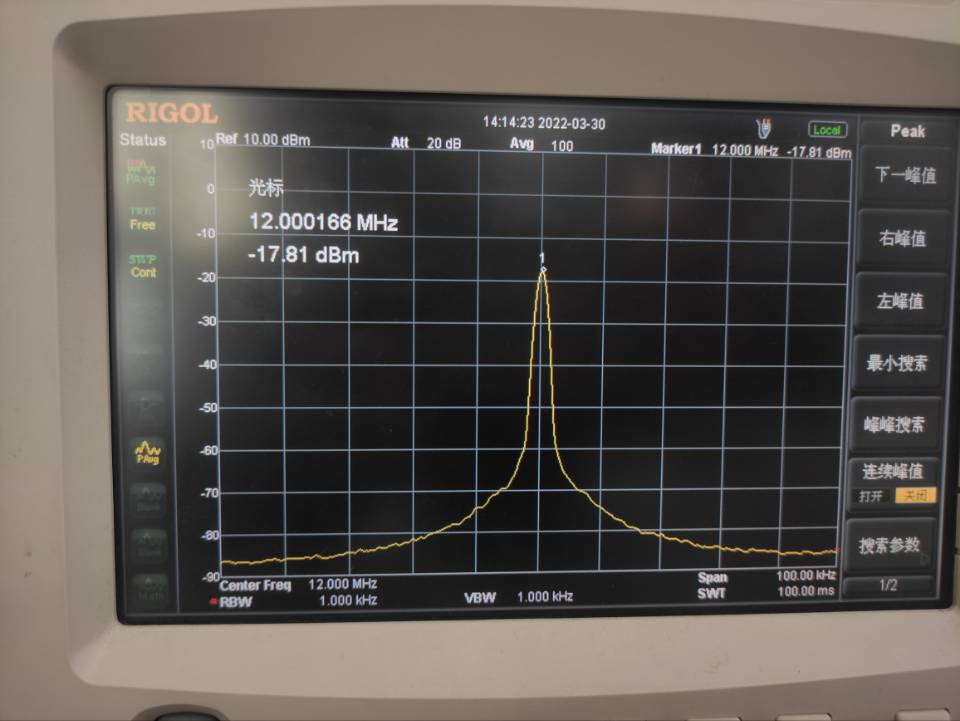
\includegraphics[width = \textwidth]{1}
            \caption{12进位选择器加法器原理图}
        \end{figure}

        \section{实验设备}
        装有Vivado、ModelSim SE软件的计算机。
        \section{实验内容}
            \subsection{实验设计}
            32位进位选择加法器的结构参考了讲义中12位进位选择加法器的设计,将加法器分成了8块,其中除去最低为的由4位超前进位加法器构成的计算块外,其余7块中间块设计如下图
            \begin{figure}[H]
                \centering
                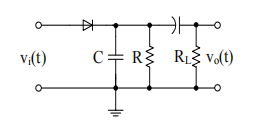
\includegraphics[width = 0.4\textwidth]{2}
                \caption{中间块设计原理图}
            \end{figure}

            \subsection{实验代码}

            \lstinputlisting[
                language = Verilog,
                title = {4位加法器代码}
            ]{src/adder_4bits.v}

            \lstinputlisting[
                language = Verilog,
                title = {32位进位选择加法器代码}
            ]{src/adder_32bits.v}

            \lstinputlisting[
                language = Verilog,
                title = {中间块设计代码}
            ]{src/csa.v}
        \section{仿真分析}
            \subsection{4位加法器仿真分析}
            \begin{figure}[H]
                \centering
                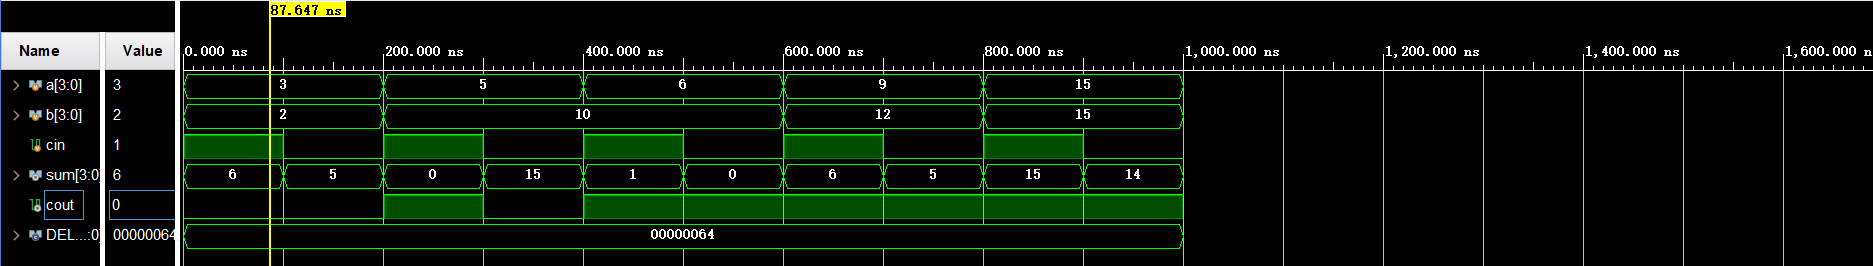
\includegraphics[width = \textwidth]{sim4_1}
                \caption{4位加法器仿真分析整体图}
            \end{figure}
            
            \begin{figure}[H]
                \centering
                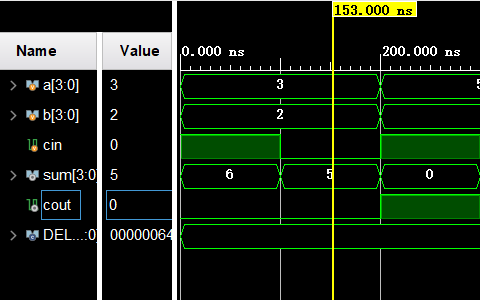
\includegraphics[width = 0.6\textwidth]{sim4_2}
                \caption{4位加法器仿真分析局部图}
            \end{figure}
            如图所示:当加数a = 3, b = 2, 进位ci = 0时,和sum = 5, 进位输出cout = 0。符合设计预期。同时,其余测试数据经检验也符合设计预期,此不在一一赘述。
            \subsection{32位进位选择器加法器仿真分析}
            \begin{figure}[H]
                \centering
                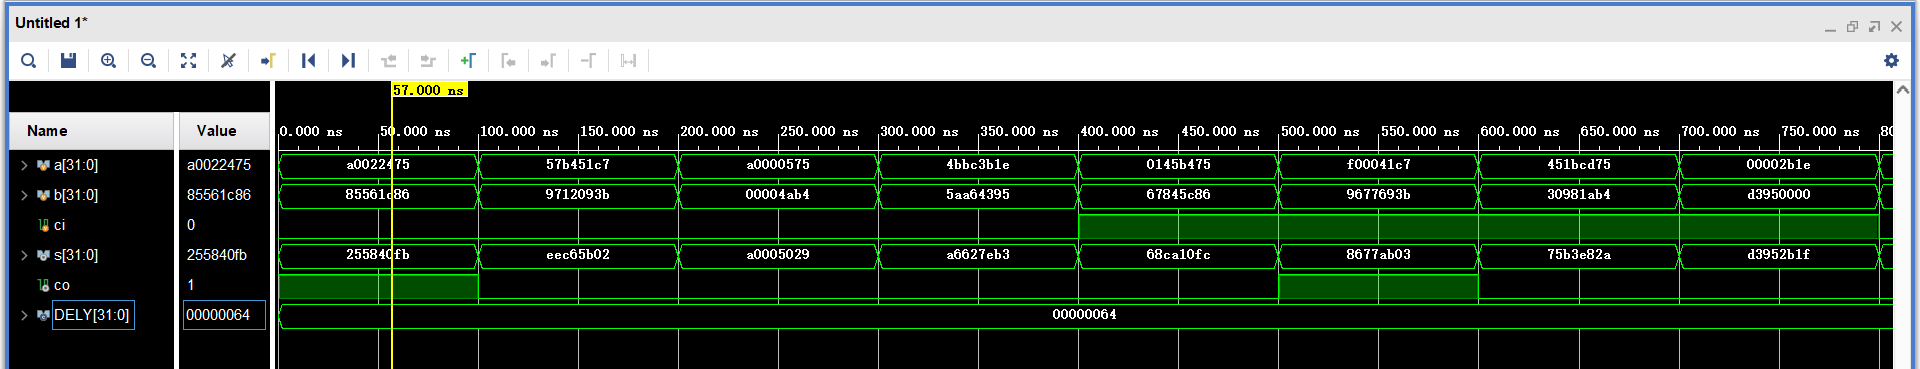
\includegraphics[width = 1\textwidth]{sim32_1}
                \caption{32位加法器仿真分析整体图}
            \end{figure}
            \begin{figure}[H]
                \centering
                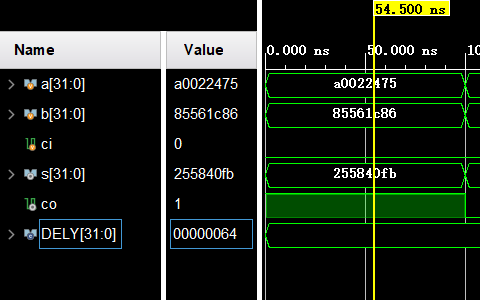
\includegraphics[width = 0.6\textwidth]{sim32_2}
                \caption{32位加法器仿真分析局部图1}
            \end{figure}
            如图所示:当加数a = 0xa0022475, b = 0x85561c86, 进位ci = 0时,和sum = 0x255740fb, 进位输出cout = 1。符合设计预期。
            \begin{figure}[H]
                \centering
                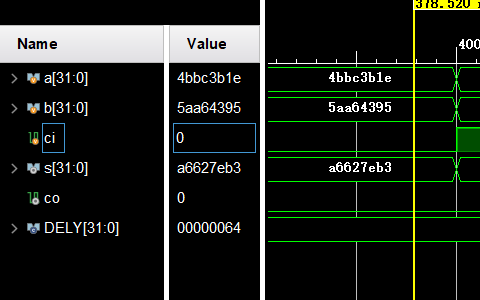
\includegraphics[width = 0.6\textwidth]{sim32_3}
                \caption{32位加法器仿真分析局部图2}
            \end{figure}
            如图所示:当加数a = 0x4bbc3b1e, b = 0x5aa64395, 进位ci = 0时,和sum = 0xa6627eb3, 进位输出cout = 0。符合设计预期。同时,其余测试数据经检验也符合设计预期,此不在一一赘述。
        \section{思考题}
            \begin{enumerate}
                \item 为什么要进行时序仿真?
                
                仿真过程是正确实现设计的关键环节,用来验证设计者的设计思想是否正确,及在设计实现过程中各种分布参数引入后,其设计的功能是否依然正确无误。
                而时序仿真使用布局布线后器件给出的模块和连线的延时信息, 在最坏的情况下对电路的行为作出实际地估价。可以比较真实地反映出器件的延时情况

                \item 采用流水线技术有什么优缺点?
                
                优点:流水线技术是将操作执行工作量分成若干个时间上均衡的操作段,从流水线的起点连续地输入,流水线的各操作段以重叠方式执行。这使得操作执行速度只与流水线输入的速度有关,而与处理所需的时间无关。这样,在理想的流水操作状态下,其运行效率很高。
                缺点:流水线会增大资源的使用。
            \end{enumerate}

\end{document}